\documentclass[a4paper, 12pt]{article}
\usepackage[top=3cm, bottom=3cm, left=2.5cm, right=2.5cm]{geometry}
\usepackage[german]{babel}
\usepackage{hyperref} % For clickable links
\usepackage{lmodern}  % Improved font rendering
\usepackage{setspace} % Adjust line spacing
\usepackage{graphicx} % For better layout options
\usepackage{titlesec} % For custom section formatting

% Title Formatting
\titleformat{\section}{\large\bfseries\centering}{\thesection}{1em}{}
\titleformat{\subsection}{\normalsize\bfseries}{\thesubsection}{1em}{}

% Custom Title
\title{\vspace{-1cm}SWEN1 - Final Protokoll MCTG}
\author{
    \textbf{Samuel Hammerschmidt} \\
    \href{https://github.com/shammerschmidt1999/SWEN1}{\texttt{GitHub: github.com/shammerschmidt1999/SWEN1}}
}
\date{Januar 2025}

\begin{document}

\maketitle

\section{Einführung}
\subsection{Projektstruktur}
Das Projekt MCTG ist in mehrere Klassen aufgeteilt. Durch Vererbung und Polymorphismus wird eine einfache Erweiterung des Spiels ermöglicht.
Die Klassen sind in verschiedene Dateien und Namespaces aufgeteilt, um die Struktur des Projekts übersichtlich zu halten. 
Weiters wurden Interfaces implementiert, um die Klassen flexibler und austauschbarer zu machen.
Neben ihren Properties besitzen Klassen auch private Fields, dies dient der Steuerung des Zugriffs auf die Eigenschaften.
Die Verwendung von Enumerationen verbessert die Lesbarkeit des Codes und ermöglicht eine einfache Erweiterung des Spiels.
Die meisten Methoden, die Zugriff auf die Datenbank benötigen oder HTTP-Anfragen verarbeiten, sind asynchron, um die Performance des Spiels zu verbessern.

\vspace{0.5cm}
\section{Klassenbeschreibung}
\subsection{User}
Die \texttt{User}-Klasse repräsentiert einen Benutzer des Spiels. Um die Daten persistent zu halten, werden User in der Datenbank gespeichert.
Die \texttt{User}-Klasse ist eine der wichtigsten und am häufigsten verwendeten Klassen im Projekt, da die meisten Operationen von dem \texttt{User} abhängen.
Änderungen an den User-Objekten werden in der Datenbank gespeichert, um die Daten konsistent zu halten, während Informationen auch direkt von der \texttt{User}-Tabelle abgerufen werden.

\subsection{Card}
Die \texttt{Card}-Klasse repräsentiert eine Karte im Spiel. Es gibt verschiedene Arten von Karten, die von der \texttt{Card}-Klasse abgeleitet sind, \texttt{MonsterCard} und \texttt{SpellCard}.
Die Karten werden in der Datenbank gespeichert und können von \texttt{Usern} gekauft und ins Deck gelegt werden. Diese Operationen werden von der \texttt{CardRepository}-Klasse durchgeführt.
Da \texttt{User}, wie in einem Trading Card Game üblich, mehrere Karten derselben Art besitzen können, wurde die Zwischentabelle \texttt{user\_cards} erstellt, die die Beziehung zwischen \texttt{Usern} und \texttt{Cards} repräsentiert.

\subsection{Battle}
Die \texttt{Battle}-Klasse repräsentiert ein \texttt{Battle} zwischen zwei \texttt{Usern}. Die Karten der \texttt{User} werden in einem \texttt{Stack} gespeichert und die Karten werden in einer Runde gespielt.
Jede Runde wird im \texttt{BattleLog} gespeichert und am Ende des Kampfes an beide \texttt{User} ausgegeben. Außerdem übernimmt der Gewinner der Runde die Karte des Verlierers.
Weiters regelt die \texttt{Battle}-Klasse die Berechnung des Schadens der Karten nach den definierten Regeln und prüft den Sieger des Kampfes.

\subsection{Package}
Ein Objekt der \texttt{Package}-Klasse repräsentiert eine Sammlung von Karten, die vom \texttt{User} mit seinen \texttt{Coins} gekauft werden können.
Ein Package speichert seinen \texttt{PackageType}, die direkten Einfluss auf den Preis, Anzahl der Karten und Anzahl der Möglichkeiten für den User definiert.

\subsection{Stack}
Ein Objekt der \texttt{Stack}-Klasse repräsentiert eine Sammlung von Karten, die einen \texttt{User} gehören. Verwendet werden \texttt{Stack}-Entitäten vor allem bei Operationen
mit den gesamten \texttt{Cards} eines \texttt{Users} und den Karten, die der \texttt{User} in seinem Deck hat. Unterschieden wird hier durch den \texttt{bool inDeck}, der bei einem \texttt{Card}-Objekt hinterlegt ist.

\subsection{CoinPurse \& Coin}
\texttt{Coins} dienen als Währung im Spiel und haben je nach \texttt{CoinType} einen anderen Wert. Die \texttt{CoinPurse}-Klasse speichert die Anzahl der \texttt{Coins} eines \texttt{Users} und ermöglicht dadurch den Kauf von \texttt{Packages}.

\section{Design- und technische Entscheidungen}
\subsection{GlobalEnums}
Die \texttt{GlobalEnums}-Klasse ist eine statische Klasse, die alle Enumerationen enthält, die im Spiel verwendet werden. Sie enthält die folgenden Enumerationen:
\begin{itemize}
    \item \texttt{ElementType}: Die Elementtypen der Karten (Fire, Water, Normal).
    \item \texttt{MonsterType}: Die Monstertypen der Monsterkarten (Dragon, Goblin, Wizard, Knight, Ork, FireElve, Kraken).
    \item \texttt{CoinType}: Die Münztypen (Diamond, Platinum, Gold, Silver, Bronze).
    \item \texttt{RoundResult}: Die Ergebnisse einer Runde (Victory, Defeat, Draw).
    \item \texttt{PackageType}: Die Typen von \texttt{Packages} (Basic, Premium, Legendary).
\end{itemize}
Die Verwendung einer globalen Klasse für die Enumerationen ermöglicht eine einfache Anwendung der Enumerationen in verschiedenen Bereichen des Spiels.
Weiters führt die Verwendung von Enumerationen zu einer verbesserten Lesbarkeit des Codes und die globale Sammlung der Enumerationen ermöglicht eine einfache Erweiterung und eine übersichtliche Struktur.

\subsection{Unit Tests}
Für die Klassen \texttt{User, Card} und \texttt{Battle} sowie für die Repositories \texttt{StackRepository} und \texttt{UserRepository} wurden Unit Tests implementiert.
Die Tests der Klassen achten vor allem auf eine richtige Initialisierung der Objekte und das korrekte Verhalten bei Änderungen der Objekteigenschaften. 
Die Tests der Repositories überprüfen die korrekte Speicherung und den korrekten Zugriff auf die Daten in der Datenbank.

\subsection{Unique Feature}
User haben die Möglichkeit, \texttt{Packages} von verschiedner Qualität zu kaufen. Im \texttt{PackageType}-Enum sind die jeweiligen Typen aufgelistet. Ein \texttt{Package} kostet bestimmt viele \texttt{Coins}, je nach Qualität.
Um die \texttt{Coins} des \texttt{Users} zu speichern, wurde die \texttt{CoinPurse}-Klasse implementiert. Das \texttt{CoinPurseRepository} und die \texttt{PackageService}-Klasse übernehmen die nötigen Schritte für den Kauf von \texttt{Packages} in der Datenbank.
\texttt{Coins} haben außerdem auch einen verschiedenen Wert, je nach \texttt{CoinType}. Dies wird im \texttt{CoinType}-Enum festgelegt.

\subsection{Trading}
Die Trading Funktionalität wurde nicht implementiert.

\subsection{Datenbank}
Die Datenbank wurde in \texttt{PostgreSQL} erstellt und beinhaltet die folgenden Tabellen:
\begin{itemize}
    \item \texttt{users}: Speichert die User-Daten.
    \item \texttt{cards}: Speichert die Karten-Daten.
    \item \texttt{user\_cards}: Speichert die Beziehung zwischen Usern und Karten.
    \item \texttt{coin\_purses}: Speichert die Coin-Daten der User.
    \item \texttt{tokens}: Speichert die Tokens der User.
\end{itemize}
Die dafür notwendigen Operationen werden von dem zugehörigen Repository durchgeführt. Diese erben alle von der Base-Klasse \texttt{RepositoryT}.
Der \texttt{Connection-String} zur Datenbank wird in einer JSON-Datei \texttt{appsettings.json} gespeichert und von der \texttt{AppSettings}-Klasse geladen.

\subsection{HTTP-Server}
Der HTTP-Server wurde implementiert, um die Anfragen der User zu ermöglichen. Der eigentlichen Operation werden in den Handlern, die von der \texttt{Handler} Basisklasse erben, durchgeführt. Folgende Handler wurden implementiert:
\begin{itemize}
    \item \texttt{UserHandler}: Verarbeitet die Erstellung, Anmeldung, Änderung und Informationsabfrage von \texttt{Usern}.
    \item \texttt{SessionHandler}: Ermöglicht die Anmeldung von \texttt{Usern}.
    \item \texttt{BattleHandler}: Ermöglicht das asynchrone Spielen von \texttt{Battles} zwischen zwei \texttt{Usern}.
    \item \texttt{PackagesHandler}: Dient zum Kauf von \texttt{Packages}.
    \item \texttt{ScoreboardHandler}: Ermöglicht das Anzeigen des Scoreboards.
    \item \texttt{CardsHandler}: Ermöglicht das Anzeigen von Karten.
    \item \texttt{DeckHandler}: Ermöglicht das Anzeigen und Bearbeiten von Decks.
    \item \texttt{StatsHandler}: Ermöglicht das Anzeigen der User-Stats.
\end{itemize}

Der HTTP-Server funktioniert folgendermaßen:
\begin{enumerate}
    \item In der \texttt{Program}-Klasse wird ein \texttt{HttpSvr}-Objekt erstellt und mittels der Methode \texttt{Run()}gestartet. Der Server lauscht auf eingehende HTTP-Anfragen.
    \item Das Incoming-Event des Servers wird mit der asynchronen Methode \texttt{Svr\_Incoming()} verknüpft, die aufgerufen wird, wenn eine Anfrage eingeht.
    \item Die Methode \texttt{Svr\_Incoming()} empfängt die Anfrage und gibt die HTTP-Methode, den Pfad und die Header der Anfrage auf der Konsole aus.
    \item Basierend auf dem Pfad der Anfrage wird entschieden, welcher \texttt{Handler} die Anfrage weiterverarbeiten soll. Dies geschieht durch die \texttt{HandleEventAsync()} Methode der \texttt{Handler}-Klasse.
    \item Sollte kein passender Handler gefunden werden, wird eine 404-Fehlermeldung zurückgegeben.
    \item Die \texttt{HttpSvrEventArgs}-Klasse enthält Informationen über die eingehende HTTP-Anfrage, einschließlich Methode, Pfad, Header und Payload.
    \item Die Methode \texttt{Reply} der \texttt{HttpSvrEventArgs}-Klasse wird verwendet, um eine HTTP-Antwort an den Client zu senden, einschließlich Statuscode und optionalem Antworttext.
\end{enumerate}

\subsection{Tokens}
Beim Einloggen eines \texttt{Users} wird ein \texttt{Token} generiert und an den Client zurückgegeben. Dieser \texttt{Token} wird im weiteren Verlauf des Projektes bei jeder Anfrage des Clients an den Server mitgeschickt und dient zur Authentifizierung des Benutzers. Der \texttt{Token} wird in der Datenbank gespeichert und mit dem \texttt{User} verknüpft. Der \texttt{Token} wird wie folgt generiert:
\begin{enumerate}
    \item Nach dem der entsprechende Endpunkt (\texttt{/sessions}) vom Client erhalten wurde, wird die \texttt{\_CreateSessionAsync()}-Methode des \texttt{SessionHandler} aufgerufen.
    \item In der Anfrage sind ein username und password string enthalten, diese werden mit den Daten in der \texttt{users} Datenbank verglichen.
    \item Bei einem Match wird die \texttt{\_CreateTokenForAsync()}-Methode der \texttt{Token}-Klasse aufgerufen, die einen zufälligen Token erstellt und in der Datenbank gespeichert. Der generierte Token wird in der Reply mitgeschickt. Ansonsten wird eine 401-Statuscode Fehlermeldung als Reply returniert.
\end{enumerate}

\subsection{Interfaces}
Für die meisten Klassen wurden Interfaces implementiert. Dies hat den Grund, dass die Klassen dadurch flexibler und austauschbarer werden. 
So kann z.B. ein \texttt{MonsterCard}-Objekt als \texttt{Card}-Objekt behandelt werden, wenn es das \texttt{ICard}-Interface implementiert. 
Dadurch können Methoden, die ein \texttt{Card}-Objekt erwarten, auch ein \texttt{MonsterCard}-Objekt akzeptieren.
Das führt zu einer verbesserten Lesbarkeit und Wartbarkeit des Codes und ermöglicht eine einfachere Erweiterung des Spiels.

\section{Lessons Learned}
\subsection{Datenbank}
Die Verwendung von \texttt{PostgreSQL} als Datenbank hat sich als gute Wahl erwiesen. Die Datenbank ist einfach zu bedienen und bietet eine gute Performance.
Weiters bietet das grafische Interface von pgAdmin 4 als Verwaltungstool eine einfache Möglichkeit, die Datenbank zu verwalten und Abfragen auszuführen.
Weiters half mir pgAdmin 4 speziell am Anfang der Datenbank-Entwicklung, da das Tool simpel zu bedienen ist und eine gute Übersicht über die Datenbankstruktur bietet.

\subsection{Unit Tests}
Die Unit Tests wurden mit dem \texttt{MSTest}-Framework implementiert. Vor allem die dadurch entstandene Trennung der Tests und des eigentlichen Codes, ermöglicht eine gute Übersicht des Repositories.
Weiters hat das kontinuierliche Entwickeln von Tests während der Funktionsimplementierung dazu geführt, dass die Klassen und Methoden besser strukturiert und getestet wurden.


\subsection{Klassenstruktur}
Die Erstellung von eigenen Klassen für spezielle Operationen, wie z.B. \texttt{AppSettings} und \texttt{PasswordHelper}, hat sich als sinnvoll erwiesen, um den Code übersichtlicher zu halten und Verwirrung zu vermeiden.

\subsection{C\# und Projektarbeit}
Zwar habe ich im Laufe meiner ersten Betriebspraxisphase bereits Erfahrung mit C\# gesammelt, jedoch war die Entwicklung eines größeren Projektes ohne ein Team eine neue Herausforderung für mich.
Durch die Entwicklung des MCTG-Projektes konnte ich meine Kenntnisse in C\# vertiefen und habe mich auch darin verbessert, ein Projekt alleine zu verwalten und auf eigenständige, für mein Projekt passende Lösungen zu finden.
\pagebreak

\section{Timetable}
\begin{table}[h!]
\centering
\begin{tabular}{|l|c|}
\hline
\textbf{Arbeitspaket} & \textbf{Zeit (Stunden)} \\ \hline
Erste Projektstruktur & 2 \\ \hline
Recherchen & 3 \\ \hline
Erste Erstellung der Klassen & 5 \\ \hline
Implementierung des HTTP-Servers & 10 \\ \hline
Erstellung Intermediate Abgabe & 5 \\ \hline
Datenbankstruktur & 7 \\ \hline
Datenbankanbindung & 2 \\ \hline
Erstellung der Repositories & 15 \\ \hline
Implementierung Unique Feature & 7 \\ \hline
Anpassung des Codes von In-Memory zu DB & 12 \\ \hline
(Unit) Testing & 6 \\ \hline
Battle \& Asynchronität & 10 \\ \hline
Final Refactoring & 8 \\ \hline
Erstellung der finalen Abgabe & 4 \\ \hline
\textbf{Summe} & \textbf{96} \\ \hline
\end{tabular}
\caption{Timetable - MCTG Projekt}
\label{tab:timetable}
\end{table}

\pagebreak

\section{UML-Diagramme}

\subsection {Class Pattern}
\noindent\textbf{Hinweis:} Hier wird nur die \texttt{Stack}-Class gezeigt, um das Pattern der Classes zu darzustellen. Der Aufbau ist für sämtliche Classes ähnlich.
\begin{figure}[h!]
\centering
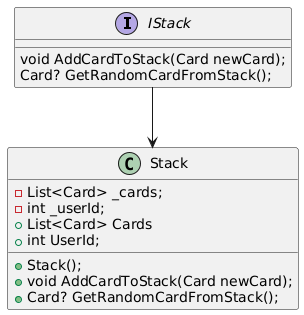
\includegraphics[width=0.8\textwidth]{Class_UML_Example_Stack.png}
\caption{UML-Diagramm des Class Patterns}
\label{fig:repository_pattern}
\end{figure}
\pagebreak

\subsection {Repository Pattern}
\noindent\textbf{Hinweis:} Hier wird nur das \texttt{UserRepository} gezeigt, um das Pattern der Repositories zu darzustellen. Der Aufbau ist für sämtliche Repositories ähnlich.
\begin{figure}[h!]
\centering
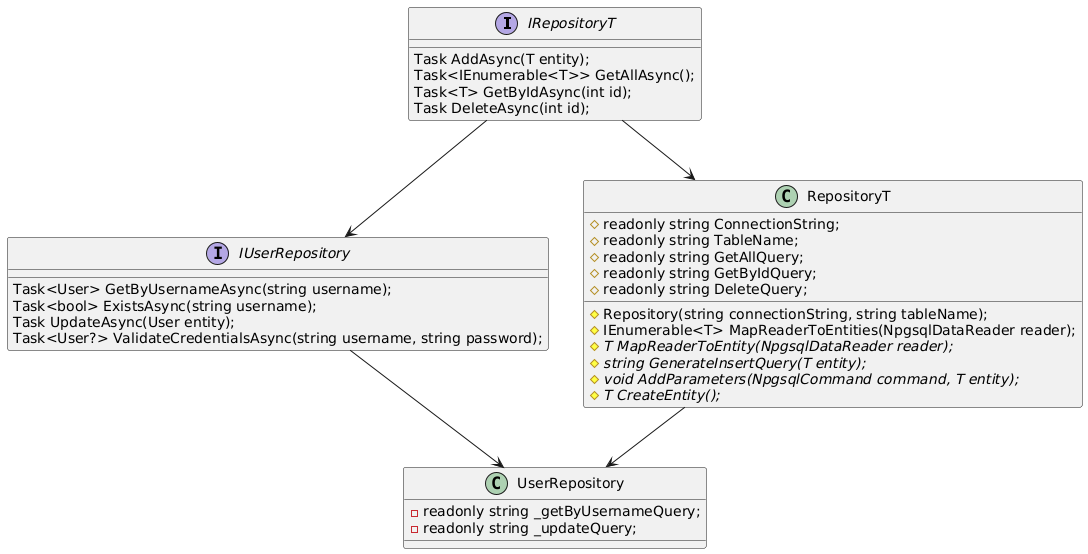
\includegraphics[width=0.8\textwidth]{Repository_UML_Example_User.png}
\caption{UML-Diagramm des Repository Patterns}
\label{fig:repository_pattern}
\end{figure}
\pagebreak

\subsection {Handler Pattern}
\noindent\textbf{Hinweis:} Hier wird nur der \texttt{UserHandler} gezeigt, um das Pattern der Handler zu darzustellen. Der Aufbau ist für sämtliche Handler ähnlich.
\begin{figure}[h!]
\centering
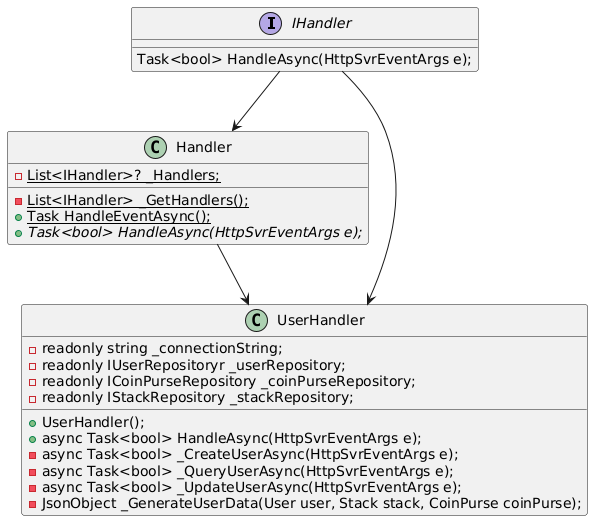
\includegraphics[width=0.8\textwidth]{Handler_UML_Example_User.png}
\caption{UML-Diagramm des Handler Patterns}
\label{fig:repository_pattern}
\end{figure}

\end{document}
